\section{Proportion et pourcentage}

\subsection{Proportion}

\begin{ex}{}
	\nline
	\begin{wrapstuff}
		\begin{tikzpicture}[scale=0.9]
			% Grand ensemble (Premières)
			\draw[thick, bleu] (0,0) ellipse (3cm and 1.8cm);
			\node[bleu, font=\bfseries\sffamily, align=center] at (1.1, 0.5) {Premières \\ $= 480$};

			% Sous-ensemble (STMG)
			\draw[thick, rouge] (-0.8, -0.2) ellipse (1.4cm and 0.9cm);
			\node[rouge, font=\bfseries\sffamily, align=center] at (-0.8, -0.2) {STMG \\ $= 108$};
		\end{tikzpicture}
	\end{wrapstuff}
	%\ew
	Sur les $480$ élèves inscrits en classe de 1$^\text{ère}$, $108$ d'entre eux sont en STMG.

	\begin{itemize}
		\item La \textbf{population totale} des élèves de 1$^\text{ère}$ compte $480$ élèves.\\C'est la population de \textbf{référence}.
		\item La \textbf{sous-population} des élèves de STMG compte $108$ élèves.
		\item La \textbf{proportion} d'élèves de STMG parmi tous les élèves de 1$^\text{ère}$ est :
	\end{itemize}

	$$p = \dfrac{108}{480} = \dfrac{9}{40} = 0,225$$

	Cette proportion peut s'exprimer en \textbf{pourcentage} : $p = 22,5 \%$.

\end{ex}

\subsection{Pourcentage d'un nombre}

\begin{prop}{}
	La proportion d'une \textbf{sous-population} (d'effectif $n$) parmi une \textbf{population totale} (d'effectif $N$) est :

	$${p=\dfrac{n}{N}}$$

	En pourcentage :

	$${p_{\%}=\dfrac{n}{N}\times 100}$$
\end{prop}

\begin{rem}
	\nline
	\begin{wrapstuff}
		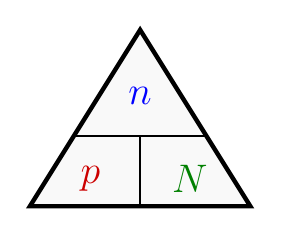
\begin{tikzpicture}[scale=0.7]
			\draw[ultra thick, fill=gray!5] (0,0) -- (4,0) -- (2,3.2) -- cycle;
			\draw[thick] (0.8,1.28) -- (3.2,1.28);
			\draw[thick] (2,0) -- (2,1.28);
			\node[font=\Large\bfseries, text=blue] at (2,2) {$n$};
			\node[font=\Large\bfseries, text=red!80!black] at (1.1,0.5) {$p$};
			\node[font=\Large\bfseries, text=green!50!black] at (2.9,0.5) {$N$};
		\end{tikzpicture}
	\end{wrapstuff}

	Pour calculer un effectif à l'aide d'une proportion, on peut utiliser :
	\[
		{n = p \times N}\quad\text{ou}\quad{N = \dfrac{n}{p}}
	\]

	\phantom{x}

	\phantom{x}

	\phantom{x}
\end{rem}

\begin{ex}{}
	Parmi les $480$ élèves de $1$\up{ère}, $15$\% ont choisi l'option anglais renforcé.

	\begin{itemize}
		\item $15 \%$ de $480$ ont choisi l'option anglais renforcé, soit :
	\end{itemize}

	\cmath{15 \% \times 480 = \dfrac{15}{100} \times 480 = 72~\text{élèves}}
\end{ex}

\newpage

\begin{methode}{Associer effectif, proportion et pourcentage}

	Une société de $75$ employés compte $12\%$ de cadres et le reste d'ouvriers.

	$35$ employés de cette société sont des femmes et $5$ d'entre elles sont cadres.

	\begin{enumerate}
		\item Calculer l'effectif des cadres.
		\item Calculer la proportion de femmes dans cette société.
		\item Calculer la proportion, en \%, de cadres parmi les femmes.\\Les femmes cadres sont-elles sous ou surreprésentées dans cette société ?
	\end{enumerate}

	\begin{correction}

		1. $12 \%$ de $75$ = $\dfrac{12}{100} \times 75 = 9.\quad$ Cette société compte $9$ cadres.

		2. La proportion de femmes est donc égale à :
		$$p_{1} = \dfrac{35}{75}= \dfrac{7}{15} \approx 0,47$$
		La société compte environ $47 \%$ de femmes.

		3. La population de référence est maintenant "les femmes".

		La proportion de cadres parmi les femmes est égale à :
		$$p_{2} =\dfrac{5}{35} = \dfrac{1}{7} \approx 0,14 = 14\%$$
		$14\% > 12\%$ donc les femmes cadres sont surreprésentées dans cette société.
	\end{correction}
\end{methode}

\subsection{Pourcentage de pourcentage}
\begin{ex}{}
	%\bw{r}{9cm}\vspace*{-10mm}
	\begin{center}
		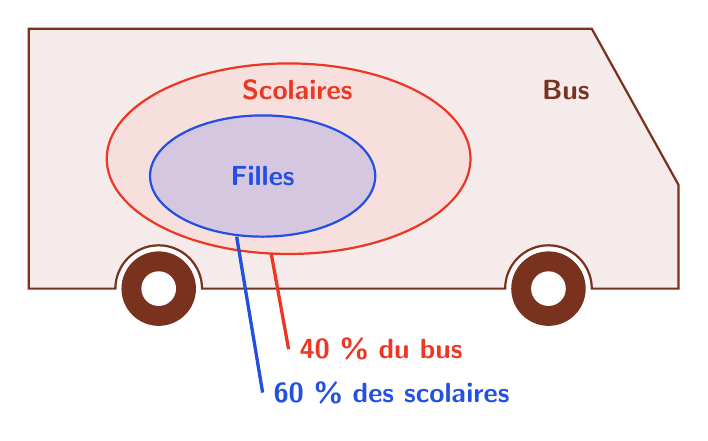
\begin{tikzpicture}[scale=1.1]
			\definecolor{busColor}{RGB}{120, 50, 30}
			\definecolor{busFill}{RGB}{245, 235, 235}
			\definecolor{scolaireColor}{RGB}{235, 55, 35}
			\definecolor{scolaireFill}{RGB}{248, 215, 210}
			\definecolor{filleColor}{RGB}{35, 80, 225}
			\definecolor{filleFill}{RGB}{200, 190, 225}
			\draw[thick, busColor, fill=busFill] (0,0) -- (1,0) arc (180:0:0.5) -- (5.5,0) arc (180:0:0.5) -- (7.5,0) -- (7.5,1.2) -- (6.5,3) -- (0,3) -- cycle;
			\fill[busColor] (1.5,0) circle (0.43);
			\fill[white] (1.5,0) circle (0.2);
			\fill[busColor] (6,0) circle (0.43);
			\fill[white] (6,0) circle (0.2);
			\node[busColor, font=\bfseries\sffamily] at (6.2, 2.3) {Bus};
			\draw[thick, scolaireColor, fill=scolaireFill, fill opacity=0.6, text opacity=1] (3, 1.5) ellipse (2.1cm and 1.1cm);
			\node[scolaireColor, font=\bfseries\sffamily] at (3.1, 2.3) {Scolaires};
			\draw[thick, filleColor, fill=filleFill, fill opacity=0.7, text opacity=1] (2.7, 1.3) ellipse (1.3cm and 0.7cm);
			\node[filleColor, font=\bfseries\sffamily] at (2.7, 1.3) {Filles};
			\draw[very thick, scolaireColor] (2.8, 0.4) -- (3, -0.7) node[right, font=\bfseries\sffamily] {40 \% du bus};
			\draw[very thick, filleColor] (2.4, 0.6) -- (2.7, -1.2) node[right, font=\bfseries\sffamily] {60 \% des scolaires};
		\end{tikzpicture}
	\end{center}
	%\ew
	Dans un bus, il y a $40\%$ de scolaires.

	Parmi les scolaires, $60\%$ sont des filles.

	La proportion de scolaires filles dans le bus est :

	$$
		\begin{aligned}
			60\%\text{ de }40\% & = 60\% \times 40\% \\
			~                   & = 0,6 \times 0,4   \\
			~                   & = 0,24 = 24 \%
		\end{aligned}
	$$

	Il y a donc $24 \%$ de filles scolaires dans le bus.
\end{ex}

\begin{prop}{}
	%\bw{r}{8cm}\vspace*{-3mm}
	\begin{center}
		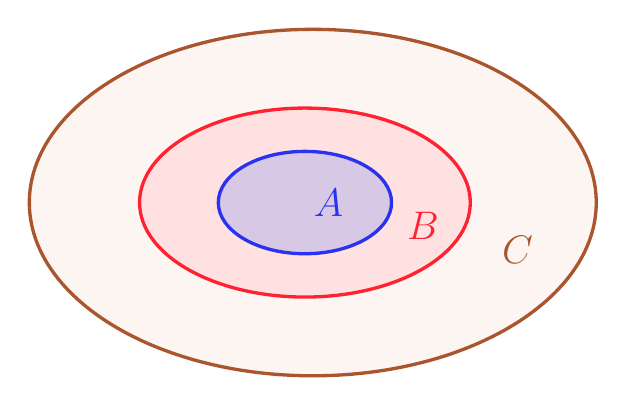
\begin{tikzpicture}
			\definecolor{cColor}{RGB}{170, 85, 45}
			\definecolor{cFill}{RGB}{252, 245, 242}
			\definecolor{bColor}{RGB}{255, 35, 50}
			\definecolor{bFill}{RGB}{255, 225, 225}
			\definecolor{aColor}{RGB}{40, 50, 240}
			\definecolor{aFill}{RGB}{215, 200, 230}
			\draw[very thick, cColor, fill=cFill] (0, 0) ellipse (3.6cm and 2.2cm);
			\node[cColor, font=\Large] at (2.6, -0.6) {$C$};
			\draw[very thick, bColor, fill=bFill] (-0.1, 0) ellipse (2.1cm and 1.2cm);
			\node[bColor, font=\Large] at (1.4, -0.3) {$B$};
			\draw[very thick, aColor, fill=aFill] (-0.1, 0) ellipse (1.1cm and 0.65cm);
			\node[aColor, font=\Large] at (0.2, 0) {$A$};
		\end{tikzpicture}
	\end{center}
	%\ew
	Soient 3 ensembles $A$ , $B$ et $C$ tel que $A\subset B$ et $B\subset C$.

	Soit :
	\begin{itemize}
		\item $p_{1}$ est la proportion de $A$ dans $B$.
		\item $p_{2}$ est la proportion de $B$ dans $C$.
	\end{itemize}

	Alors $\quad{p_{1} \times p_{2}}\quad$ est la proportion de $A$ dans $C$.
	\vspace*{22mm}
\end{prop}

\begin{rem}{}
	Pour calculer \textbf{un pourcentage de pourcentage}, on multiplie les pourcentages entre eux.
\end{rem}
\newpage

\begin{methode}{Calculer un pourcentage de pourcentage}
	%%\bw{r}{9cm}\vspace*{-5mm}\cimg{9cm}{img/cours/04.png}\vspace*{-25mm}\ew
	Sur $67$ millions d'habitants en France, $66\%$ de la population est en âge de travailler (15-64 ans).

	La population active représente $70\%$ de la population en âge de travailler.
	\be
	\item Calculer la proportion de population active par rapport à la population totale.
	\item Combien de français compte la population active ?
	\ee

	\vspace*{10mm}

	\begin{correction}

		1. Le pourcentage de population active par rapport à la population totale est égal à :
		\cmath{
			\begin{array}{rcll}
				p & = & p_1 \times p_2          &                  \\
				  & = & 70 \% \text{ de } 66 \% &                  \\
				  & = & 0,7 \times 0,66         & = 0,462 = 46,2\%
			\end{array}
		}
		On a donc $46,2\%$ des français sont actifs.

		\smallskip

		2. On a :

		\cmath{
			\begin{array}{rcll}
				n & = & p\times N           &          \\
				  & = & 46,2\%\text{ de }67 &          \\
				  & = & 0,462 \times 67     & = 30,954
			\end{array}
		}

		La France compte environ $31$ millions d'actifs.

	\end{correction}
\end{methode}

\section{Fréquence conditionnelle, fréquence marginale}
\subsection{Définition et méthode de calcul}
\begin{defin}{Fréquence marginale, fréquence conditionnelle}
	Dans un tableau croisé d'effectifs (ou tableau à double entrée) :

	\ms
	\begin{center}
		\begin{tabular}{|r|c|c||c|} \hline
			\rowcolor{gray!15} \phantom{Caractère $A$}                                         & Caractère $B_1$ & Caractère $B_2$ & Total \\ \hline
			Caractère $A_1$                                                                    &
			\begin{tabular}{c} Effectif \\ \textit{(Intersection)} \end{tabular}               &
			\begin{tabular}{c} Effectif \\ \textit{(Intersection)} \end{tabular}               &
			\cellcolor{blue!15}\begin{tabular}{c} Total ligne \\ \textbf{(Marge)} \end{tabular}                                            \\ \hline
			Caractère $A_2$                                                                    &
			\begin{tabular}{c} Effectif \\ \textit{(Intersection)} \end{tabular}               &
			\begin{tabular}{c} Effectif \\ \textit{(Intersection)} \end{tabular}               &
			\cellcolor{blue!15}\begin{tabular}{c} Total ligne \\ \textbf{(Marge)} \end{tabular}                                            \\ \hline\hline
			Total                                                                              &
			\cellcolor{blue!15}\begin{tabular}{c} Total col. \\ \textbf{(Marge)} \end{tabular} &
			\cellcolor{blue!15}\begin{tabular}{c} Total col. \\ \textbf{(Marge)} \end{tabular} &
			\cellcolor{purple!20}\begin{tabular}{c} \textbf{Effectif} \\ \textbf{Total $N$} \end{tabular}                                  \\ \hline
		\end{tabular}
	\end{center}

	\begin{itemize}
		\item Une \textbf{fréquence marginale} est la fréquence d'un des caractères de l'ensemble de la population.\\Elle se calcule en divisant un effectif total d'une ligne ou d'une colonne (situé en \textbf{marge} du tableau) par l'effectif total de la population.
	\end{itemize}
	\ms
	$$\text{Fréquence marginale} = \dfrac{\text{Effectif total d'une ligne ou colonne}}{\text{Effectif total}}$$
	\smallskip
	\begin{itemize}
		\item Une \textbf{fréquence conditionnelle} est la fréquence d'un caractère calculée non pas sur la population totale, mais sur une sous-population (qui définit la \textbf{condition}).\\Elle se calcule en divisant l'effectif de l'intersection (à l'intérieur du tableau) par l'effectif total de la sous-population considérée.
	\end{itemize}
	\ms
	$$\text{Fréquence conditionnelle (parmi les } A) = \dfrac{\text{Effectif de \og{}}A\text{ et }B\text{\fg{}}}{\text{Effectif total de } A}$$
\end{defin}

\newpage

\begin{methode}{Calculer une \textbf{fréquence conditionnelle}, une \textbf{fréquence marginale}}

	Dans une entreprise qui compte $360$ employés, on compte :
	\begin{itemize}
		\item $60\%$ d'hommes et parmi ceux-là, $12,5\%$ sont des cadres.
		\item Par ailleurs, $87,5\%$ des femmes de cette entreprise sont ouvrières.
	\end{itemize}

	\begin{enumerate}
		\item À l'aide des données de l'énoncé, compléter un tableau d'effectifs.
		\item Calculer \ul{la fréquence marginale} de cadres dans cette entreprise.
		\item Calculer \ul{la fréquence conditionnelle} d'ouvriers \ul{parmi les hommes}.
	\end{enumerate}
	\begin{correction}

		\begin{enumerate}
			\item Avec l'énoncé, le tableau d'effectif est le suivant :
			      $$
				      \def\arraystretch{1.2}
				      \begin{array}{|r|c|c|c|} \hline
					      \text{}         & \text{Hommes}          & \text{Femmes}           & \text{Total}    \\ \hline
					      \text{Cadres}   & 12,5\% \times 216 = 27 & 144 - 126 = 18          & 27 + 18 = 45    \\ \hline
					      \text{Ouvriers} & 216 - 27 = 189         & 87,5\% \times 144 = 126 & 189 + 126 = 315 \\ \hline
					      \text{Total}    & 60\% \times 360 = 216  & 360 - 216 = 144         & 360             \\ \hline
				      \end{array}
			      $$

			\item La \textbf{\ul{fréquence marginale}} se lit en \ul{"marge"} du tableau.
			      $$
				      \def\arraystretch{1.2}
				      \begin{array}{|r|c|c|>{\columncolor{blue!15}}c|} \hline
					      \text{}         & \text{Hommes} & \text{Femmes} & \text{Total}      \\ \hline
					      \text{Cadres}   & 27            & 18            & {\color{blue}45}  \\ \hline
					      \text{Ouvriers} & 189           & 126           & 315               \\ \hline
					      \text{Total}    & 216           & 144           & {\color{blue}360} \\ \hline
				      \end{array}
			      $$

			      On compte $360$ employés en tout et $45$ sont des cadres.

			      La \textbf{\ul{fréquence marginale}} de cadres est donc égale à :

			      $$\dfrac{45}{360} = 0,125 = 12,5 \%$$

			\item La \textbf{\ul{fréquence conditionnelle}} restreint l'effectif total.

			      Ici, on ne considère que les hommes car la "condition" est \ul{"parmi les hommes"}.

			      La \textbf{\ul{fréquence conditionnelle}} se lit sur \textbf{une ligne ou une colonne intérieure} du tableau.

			      Ici, on ne va donc considérer que la colonne concernant les hommes (condition).

			      $$
				      \def\arraystretch{1.2}
				      \begin{array}{|r|>{\columncolor{red!15}}c|c|c|} \hline
					      \text{}         & \text{Hommes}    & \text{Femmes} & \text{Total} \\ \hline
					      \text{Cadres}   & 27               & 18            & 45           \\ \hline
					      \text{Ouvriers} & {\color{red}189} & 126           & 315          \\ \hline
					      \text{Total}    & {\color{red}216} & 144           & 360          \\ \hline
				      \end{array}
			      $$

			      On compte $216$ hommes en tout et parmi eux, $189$ sont des ouvriers.

			      La fréquence \textbf{conditionnelle d'ouvriers, techniciens} parmi \ul{les hommes} est :

			      $$\dfrac{189}{216} = 0,875 = 87,5 \%$$
		\end{enumerate}
	\end{correction}
\end{methode}
\end{document}
